%%%%%%%%%%%%%%%%%%%%%%%%%%%%%%%%%%%%

\section{4.3. Testando hipóteses}

%%%%%%%%%%%%%%%%%%%%%%%%%%%%%%%%%%%%

\subsection{Quadro de testes de hipóteses}

%%%%%%%%%%%%%%%%%%%%%%%%%%%%%%%%%%%%

\begin{frame}
\frametitle{Lembre-se de quando...}
\justifying
Experimento sobre discriminação de gênero:
Ser promovido no emprego independe do gênero?

{\small
\begin{tabular}{ll  cc c} 
  		&				& \multicolumn{2}{c}{\textit{Promoção}} \\
\cline{3-4}
							&			& Promovido	& Não Promovido	& Total	\\
\cline{2-5}
\multirow{2}{*}{\textit{Gênero	}}	&Masculino 		& 21	 	& 3		& 24 	\\
							&Feminino		& 14	 	& 10 	 	& 24 \\
\cline{2-5}
							&Total		& 35		& 13		& 48 \\
\end{tabular}
}

\pause
\justifying
\[ \hat{p}_{homens} = 21 / 24 \approx 0.88 \]
\justifying
\[ \hat{p}_{mulheres} = 14 / 24 \approx 0.58 \]

\pause
\end{frame}
%%%%%%%%%%%%%%%%%%%%%%%%%%%%%%%%%%%%

\begin{frame}
\frametitle{Lembre-se de quando...}
Explicações possíveis:
\begin{itemize}
\justifying
\item Promoção e gênero são \hl{independentes}, não há discriminação de gênero, a diferença observada nas proporções é simplesmente devido ao acaso. $\rightarrow$ \orange{nulo} - {\small (nada está acontecendo)}
\justifying
\item Promoção e gênero são \hl{dependentes}, há discriminação de gênero, a diferença observada nas proporções não se deve ao acaso. $\rightarrow$ \orange{alternativa} - {\small (algo está acontecendo)}

\end{itemize}

\end{frame}

%%%%%%%%%%%%%%%%%%%%%%%%%%%%%%%%%%%%

\begin{frame}
\frametitle{Resultado}

\begin{center}
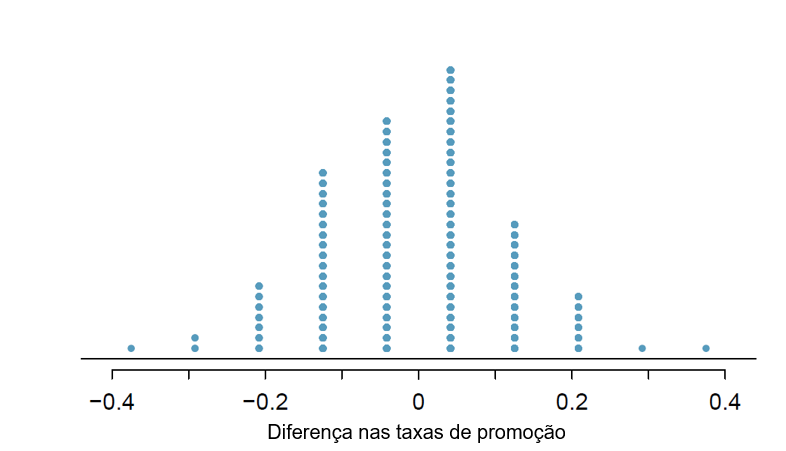
\includegraphics[width=0.6\textwidth]{4-3_hyp_test/discRandDotPlot.png}
\end{center}

\pause
\justifying
Como era bastante improvável obter resultados como os dados reais ou algo mais extremo nas simulações (promoções masculinas sendo 30\% ou mais frequentes às promoções femininas), decidimos rejeitar a hipótese nula em favor da alternativa.

\end{frame}

%%%%%%%%%%%%%%%%%%%%%%%%%%%%%%%%%%%%

\begin{frame}
\frametitle{Recapitulação: estrutura de teste de hipóteses}

\begin{itemize}
\justifying
\item Começamos com uma \hl{hipótese nula ($ H_0 $)} que representa o status quo.
\pause
\justifying
\item Também temos uma hipótese \hl{alternativa ($ H_A $)} que representa nossa questão de pesquisa, ou seja, o que estamos testando.
\pause
\justifying
\item Realizamos um teste de hipóteses sob o pressuposto de que a hipótese nula é verdadeira, seja através de simulação ou métodos tradicionais baseados no teorema do limite central (veremos logo mais...).
\end{itemize}
\end{frame}

%%%%%%%%%%%%%%%%%%%%%%%%%%%%%%%%%%%%

\begin{frame}
\frametitle{Recapitulação: estrutura de teste de hipóteses}

\begin{itemize}
\justifying
\item Se os resultados do teste sugerirem que os dados não fornecem evidências convincentes para a hipótese alternativa, nós ficaremos com a hipótese nula. Mas se o fizerem, rejeitamos a hipótese nula em favor da alternativa.
\end{itemize}
\pause
\justifying
Vamos introduzir formalmente a estrutura de testes de hipóteses usando um exemplo para testar uma afirmação sobre uma média populacional.

\end{frame}

%%%%%%%%%%%%%%%%%%%%%%%%%%%%%%%%%%%%

\subsection{Testando hipóteses usando intervalos de confiança} 

%%%%%%%%%%%%%%%%%%%%%%%%%%%%%%%%%%%%

\begin{frame}
\frametitle{Testando hipóteses usando intervalos de confiança}
\justifying
\dq{Anteriormente, calculamos um intervalo de confiança de 95\% para o número médio de relacionamentos exclusivos em que os estudantes universitários estiveram (2,7, 3,7). Com base nesse intervalo de confiança, esses dados confirmam a hipótese de que os estudantes universitários, em média, já estiveram em mais de três relacionamentos exclusivos.}

\pause

\begin{itemize}
\justifying
\item As hipóteses associadas são:
\begin{itemize}
\justifying
\item[$H_0$:] $\mu = 3$: Os estudantes universitários já estiveram em três relacionamentos exclusivos, em média.
\justifying
\item[$H_A$:] $\mu > 3$: Os estudantes universitários já estiveram em mais de 3 relacionamentos exclusivos, em média.
\end{itemize}
\end{itemize}

\end{frame}
%%%%%%%%%%%%%%%%%%%%%%%%%%%%%%%%%%%%

\begin{frame}
\frametitle{Testando hipóteses usando intervalos de confiança}

\begin{itemize}
\justifying
\item Como o valor nulo está dentro do intervalo, não rejeitamos a hipótese nula em favor da alternativa.

\pause
\justifying
\item Esta é uma abordagem rápida (e um pouco tosca) para fazer testes de hipóteses. No entanto, ela não nos diz a probabilidade de certos resultados sob a hipótese nula, ou seja, o p-valor, com base no qual podemos tomar uma decisão sobre as hipóteses.

\end{itemize}

\end{frame}

%%%%%%%%%%%%%%%%%%%%%%%%%%%%%%%%%%%%

\begin{frame}
\frametitle{Número de pedidos de faculdade}
\justifying
\dq{{\small Uma pesquisa semelhante perguntou para 206 alunos da Duke University para quantas faculdades eles aplicaram. Esta amostra rendeu uma média de 9,7 aplicações universitárias com um desvio padrão de 7. O site do College Board afirma que os orientadores recomendam que os alunos se inscrevam em aproximadamente 8 faculdades. Esses dados fornecem evidências convincentes de que o número médio de faculdades aos quais os alunos da Duke se candidatam é \emph{superior} ao recomendado?}}

\vfill
\justifying
\ct{\webURL{http://www.collegeboard.com/student/apply/the-application/151680.html}}

\end{frame}

%%%%%%%%%%%%%%%%%%%%%%%%%%%%%%%%%%

\begin{frame}
\frametitle{Definindo as hipóteses}

\begin{itemize}
\justifying
\item O \hl{parâmetro de interesse} é o número médio de escolas aplicadas por \underline{todos} estudantes da Duke.

\pause
\justifying
\item Pode haver duas explicações para a nossa média de amostra ser maior do que as 8 faculdades recomendadas.
\begin{itemize}
\justifying
\item A verdadeira média populacional é diferente.
\justifying
\item A média real da população é 8, e a diferença entre a média real da população e a média da amostra é simplesmente devido à variabilidade natural da amostragem.
\end{itemize}

\pause
\end{itemize}

\end{frame}
%%%%%%%%%%%%%%%%%%%%%%%%%%%%%%%%%%

\begin{frame}
\frametitle{Definindo as hipóteses}

\begin{itemize}
\justifying
\item Começamos com a suposição de que o número médio de faculdades em que os alunos da Duke se candidatam é 8 (como recomendado)
\[ \mathhl{H_0:}~\mu = 8 \]

\pause
\justifying
\item Testamos a alegação de que o número médio de faculdades em que os alunos da Duke se candidatam é maior que 8
\[ \mathhl{H_A:}~\mu > 8 \]

\end{itemize}

\end{frame}

%%%%%%%%%%%%%%%%%%%%%%%%%%%%%%%%%%%

\subsection{Condições para inferência}

%%%%%%%%%%%%%%%%%%%%%%%%%%%%%%%%%%%

\begin{frame}
\frametitle{Número de candidaturas universitárias - condições}
\justifying
\pq{Qual das seguintes opções \emph{não} é uma condição que precisa ser atendida para aplicar este teste de hipótese?}

\begin{enumerate}[(a)]
\justifying
\item Os alunos da amostra devem ser independentes uns dos outros em relação a quantas faculdades se candidataram.
\justifying
\item A amostragem deveria ter sido feita aleatoriamente.
\justifying
\item O tamanho da amostra deve ser menor que 10 \% da população de todos os alunos da Duke.
\justifying
\solnMult{ Deve haver pelo menos 10 sucessos e 10 falhas na amostra.}
\justifying
\item A distribuição do número de faculdades em que os alunos aplicaram não deve ser extremamente assimétrica.
\end{enumerate}

\end{frame}

%%%%%%%%%%%%%%%%%%%%%%%%%%%%%%%%%%

\subsection{Teste formal usando valores p}

%%%%%%%%%%%%%%%%%%%%%%%%%%%%%%%%%%%%

\begin{frame}
\frametitle{Estatística de teste}
\justifying
Para avaliar se a média da amostra observada é diferente da distribuição de amostragem hipotética, determinamos quantos erros-padrão podem estar fora da hipótese nula, o que também é chamado de \hl{estatística de teste}.


\pause

\twocol{0.55}{0.45}{
\begin{center}
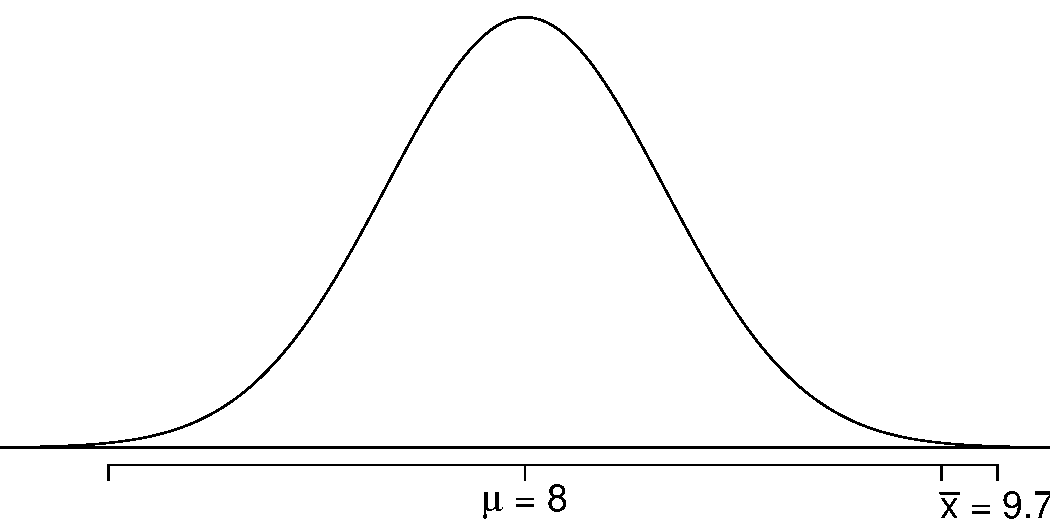
\includegraphics[width=\textwidth]{4-3_hyp_test/app_z.pdf}
\end{center}
\pause
\[ \bar{x} \sim N \pr{ \mu = 8, SE = \frac{7}{\sqrt{206}} = 0.5 } \]
\pause
\[ Z = \frac{9.7 - 8}{0.5} = 3.4 \]
}
{
\pause
\justifying
\tiny{\dq{A média da amostra é de 3,4 erros padrão longe do valor hipotético. Isso é considerado excepcionalmente alto? Ou seja, é o resultado \hl{estatisticamente significativo}?}
\pause
\justifying
\soln{Sim, e podemos quantificar o quão incomum é essa média usando um p-valor.}
}}

\end{frame}

%%%%%%%%%%%%%%%%%%%%%%%%%%%%%%%%%%%

\begin{frame}
\frametitle{P-valor}

\begin{itemize}
\justifying
\item Em seguida, usamos essa estatística de teste para calcular o \hl{p-valor}, ou seja, a probabilidade de observar dados tão favoráveis à hipótese alternativa quanto nosso conjunto de dados atual, se a hipótese nula fosse verdadeira.


\pause
\justifying
\item Se o p-valor for \hl{baixo} (menor que o nível de significância, $\alpha$, que normalmente é de 5\%), dizemos que seria muito improvável observar os dados se a hipótese nula fosse verdadeira, e daí \hl{rejeitamos $H_0$}.

\pause
\justifying
\item Se o p-valor for \hl{alto} (maior que $\alpha$), dizemos que é provável observar os dados mesmo que a hipótese nula seja verdadeira e, portanto, \hl{não rejeitamos $H_0$}.

\end{itemize}

\end{frame}

%%%%%%%%%%%%%%%%%%%%%%%%%%%%%%%%%%%%

\begin{frame}
\frametitle{Número de inscrições em faculdades - p-valor}
\justifying
\hl{P-valor:} probabilidade de observar dados pelo menos tão favoráveis a $H_A$ como nosso conjunto de dados atual (uma média de amostra maior que 9,7), se de fato $H_0$ fosse verdadeira (a média real da população é 8).


\begin{center}
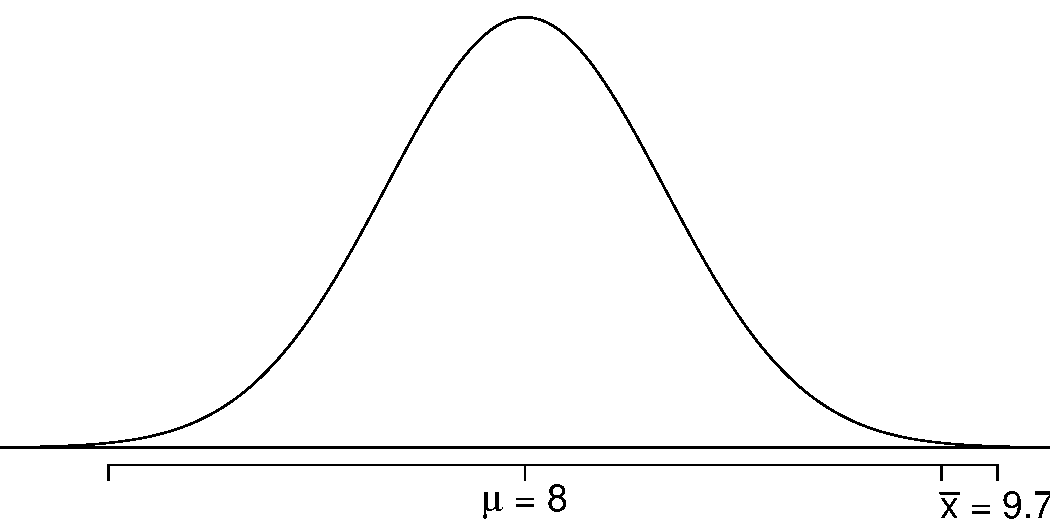
\includegraphics[width=0.55\textwidth]{4-3_hyp_test/app_pval_gr.pdf}
\end{center}

\pause

\[ P(\bar{x} > 9.7~|~\mu = 8) = P(Z > 3.4) = 0.0003 \]

\end{frame}

%%%%%%%%%%%%%%%%%%%%%%%%%%%%%%%%%%

\begin{frame}
\frametitle{Número de inscrições em faculdades - tomada de decisão}

\begin{itemize}
\justifying
\item p-valor = 0.0003

\pause

\begin{itemize}
\justifying
\item Se a média real do número de faculdades em que os alunos da Duke se candidataram é 8, há apenas 0,03\% de chance de observar uma amostra aleatória de 206 alunos da Duke que, em média, aplicaram para 9,7 ou mais faculdades.

\pause
\justifying
\item Esta é uma probabilidade muito baixa para acreeditarmos que uma média amostral de 9,7 ou mais faculdades acontecerá por acaso.
\end{itemize}

\pause
\justifying
\item Como o p-valor é \orange{baixo} (menor que 5\%), nós \orange {rejeitamos $H_0$}.

\pause
\justifying
\item Os dados fornecem evidências convincentes de que os alunos da Duke aplicaram para mais de 8 faculdades, em média.

\pause
\justifying
\item A diferença entre o a hipótese nula de 8 faculdades e a média amostral observada de 9,7 faculdades \orange{não é por acaso} ou devido à variabilidade amostral.

\end{itemize}

\end{frame}

%%%%%%%%%%%%%%%%%%%%%%%%%%%%%%%%%%%%

\begin{frame}
\frametitle{Prática}
\justifying
\pq{ Uma pesquisa da National Sleep Foundation descobriu que os estudantes universitários têm em média 7 horas de sono por noite. Uma amostra de 169 estudantes universitários que fizeram uma aula de estatística introdutória rendeu uma média de 6,88 horas de sono por noite, com um desvio padrão de 0,94 horas. Supondo que esta seja uma amostra aleatória representativa de todos os estudantes universitários {\scriptsize \textit{(com um pouco de fé?)}}, um teste de hipótese foi realizado para avaliar se os estudantes universitários em média dormem \emph{menos que} 7 horas por noite. O p-valor para este teste de hipótese é 0,0485. Qual das seguintes opções está correta?}
\end{frame}
%%%%%%%%%%%%%%%%%%%%%%%%%%%%%%%%%%%%%%%
\begin{frame}
\frametitle{Prática}
\begin{enumerate}[(a)]
\justifying
\item Não rejeitamos $H_0$, os dados fornecem evidências convincentes de que os estudantes universitários dormem em média menos de 7 horas.
\justifying
\solnMult{ Rejeitamos $H_0$, os dados fornecem evidências convincentes de que os estudantes universitários dormem menos de 7 horas em média. }
\justifying
\item Rejeitamos $H_0$, os dados provam que os estudantes universitários dormem mais de 7 horas em média.
\justifying
\item Não rejeitamos $H_0$, os dados não fornecem evidências convincentes de que os estudantes universitários dormem menos de 7 horas em média.
\justifying
\item Rejeitamos $H_0$, os dados fornecem evidências convincentes de que os estudantes universitários nesta amostra dormem menos de 7 horas em média.
\end{enumerate}

\end{frame}

%%%%%%%%%%%%%%%%%%%%%%%%%%%%%%%%%

\subsection{Teste de hipóteses bilateral e p-valor}

%%%%%%%%%%%%%%%%%%%%%%%%%%%%%%%%%

\begin{frame}
\frametitle{Teste de hipóteses bilateral e p-valor}

\begin{itemize}
\justifying
\item Se a pergunta de pesquisa for "Os dados fornecem evidências convincentes de que a média de sono dos estudantes universitários por noite é \orange{diferente} que a média nacional?", a hipótese alternativa seria diferente.
\begin{align*}
H_0&: \mu = 7 \\
H_A&: \mu \orange{~$\ne$~} 7
\end{align*}

\pause
\justifying
\item Portanto, o p-valor também mudaria:
\twocol{0.55}{0.45}
{
\begin{center}
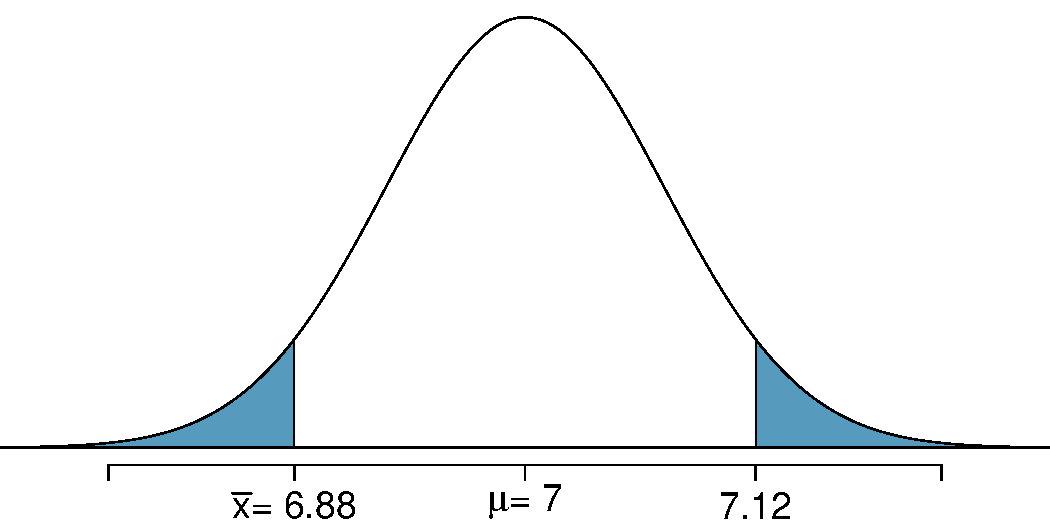
\includegraphics[width=\textwidth]{4-3_hyp_test/sleep_pval_ts.pdf}
\end{center}
}
{
\small{valor-p \\
$= 0.0485 \times 2$ \\
$= 0.097$
}}

\end{itemize}

\end{frame}

%%%%%%%%%%%%%%%%%%%%%%%%%%%%%%%%%%%%

\subsection{Erros de decisão}

%%%%%%%%%%%%%%%%%%%%%%%%%%%%%%%%%%%%

\begin{frame}
\frametitle{Erros de decisão}

\begin{itemize}
\justifying
\item Testes de hipóteses não são perfeitos.
\justifying
\item No sistema judiciário, pessoas inocentes são às vezes erroneamente condenadas e os culpados às vezes saem impunes.
\justifying
\item Da mesma forma, podemos tomar uma decisão errada nos testes de hipóteses estatísticas.
\justifying
\item A diferença é que temos as ferramentas necessárias para quantificar a frequência com que cometemos erros nas estatísticas.

\end{itemize}

\end{frame}

%%%%%%%%%%%%%%%%%%%%%%%%%%%%%%%%%%%%

\begin{frame}
\frametitle{Erros de decisão (cont.)}
\justifying
Existem duas hipóteses concorrentes: a nula e a alternativa. Em um teste de hipótese, tomamos uma decisão sobre o que pode ser verdade, mas nossa escolha pode estar incorreta. \\

\pause

\begin{center}
\begin{tabular}{l l | c c}
\multicolumn{2}{c}{} & \multicolumn{2}{c}{\textbf{Decisão}} \\
& & não rejeitar $H_0$ &  rejeitar $H_0$ \\
  \cline{2-4}
& $H_0$ verdadeiro & \onslide<3->{\green{$\checkmark$}} &  \onslide<5->{\orange{Erro tipo 1}} \\
\raisebox{1.5ex}{\textbf{Verdade}} & $H_A$ verdadeiro & \onslide<6->{\orange{Erro tipo 2}} & \onslide<4->{\green{$\checkmark$}} \\
  \cline{2-4}
\end{tabular}
\end{center}

\begin{itemize}
\justifying
\item \onslide<5->{O \hl{erro tipo 1} é quando rejeitamos a hipótese nula quando, na verdade, $H_0$ é verdadeiro.}
\justifying
\item \onslide<6->{O \hl {erro tipo 2} é quando não conseguimos rejeitar a hipótese nula quando, na verdade, $H_A$ é verdadeiro.}
\justifying
\item \onslide<7->{Nós (quase) nunca sabemos se $H_0$ ou $H_A$ é a verdade, mas precisamos considerar todas as possibilidades.}

\end{itemize}

\end{frame}

%%%%%%%%%%%%%%%%%%%%%%%%%%%%%%%%%%%%

\begin{frame}
\frametitle{Teste de Hipótese como um julgamento}
\justifying
Se pensarmos novamente em um teste de hipótese como um processo criminal, então faz sentido enquadrar o veredito em termos das hipóteses nula e alternativa:
\begin{align*}
H_0&:\text{ Réu é inocente} \\
H_A&:\text{ Réu é culpado}
\end{align*}
\justifying
Qual tipo de erro está sendo cometido nas seguintes circunstâncias?

\begin{itemize}
\justifying
\item Declarando o réu inocente quando ele é culpado.
\justifying
\soln{\only<2->{\begin{center}\hl{Erro tipo 2}\end{center}}}
\justifying
\item Declarando o réu culpado quando ele é inocente.
\justifying
\soln{\only<3->{\begin{center}\hl{Erro tipo 1}\end{center}}}
\end{itemize}
\justifying
\only<4->{Qual erro você acha que é pior?}
\justifying
\only<5>{\begin{center}{\footnotesize ``melhor dez pessoas culpadas escaparem do que um inocente sofrer''\\ -- William Blackstone}\end{center}}
\end{frame}

%%%%%%%%%%%%%%%%%%%%%%%%%%%%%%%%%%%%

\begin{frame}
\frametitle{Taxa de erro de tipo 1}

\begin{itemize}
\justifying
\item Como regra geral, rejeitamos $H_0$ quando o p-valor é menor que 0,05, ou seja, usamos um \hl{nível de significância} de 0,05, \mathhl{\alpha = 0.05}.

\pause
\justifying
\item Isso significa que, nos casos em que $H_0$ é realmente verdadeira, não queremos rejeitá-la incorretamente mais de 5\% dessas vezes. 

\pause
\justifying
\item Em outras palavras, ao usar um nível de significância de 5\%, há cerca de 5\% de chance de gerar um erro de Tipo 1 se a hipótese nula for verdadeira.
\[ \mathhl{ P(\text{Erro tipo 1 | $H_0$ Verdade}) = \alpha } \]

\pause
\justifying
\item É por isso que preferimos valores pequenos de $\alpha$ -- aumentando $\alpha$ aumenta a taxa de erro do tipo 1.

\end{itemize}

\end{frame}

%%%%%%%%%%%%%%%%%%%%%%%%%%%%%%%%%%%%

\subsection{Escolhendo um nível de significância}

%%%%%%%%%%%%%%%%%%%%%%%%%%%%%%%%%%%%

\begin{frame}
\frametitle{Escolhendo um nível de significância}

\begin{itemize}
\justifying
\item Escolher um nível de significância para um teste é importante em muitos contextos, e o nível tradicional é de 0,05. No entanto, geralmente é útil ajustar o nível de significância com base no que se está testando. 
\justifying
\item Podemos selecionar um nível menor ou maior que 0,05, dependendo das consequências de quaisquer conclusões obtidas no teste.
\justifying
\item Se as consequências de um Erro Tipo 1 forem perigosas ou caras, devemos escolher um nível de significância pequeno (por exemplo, 0,01). Sob este cenário, queremos ser muito cautelosos ao rejeitar a hipótese nula, então exigimos evidências muito fortes favorecendo $H_A$ antes de rejeitarmos $H_0$.
\end{itemize}

\end{frame}

%%%%%%%%%%%%%%%%%%%%%%%%%%%%%%%%%%%%

\begin{frame}
\frametitle{Escolhendo um nível de significância}

\begin{itemize}
\justifying
\item Se um Erro Tipo 2 for relativamente mais perigoso ou muito mais dispendioso do que um Erro Tipo 1, então devemos escolher um nível de significância mais alto (por exemplo, 0,10). Aqui, queremos ter cautela ao não rejeitar $H_0$ quando a hipótese nula for realmente falsa.

\end{itemize}

\end{frame}

%%%%%%%%%%%%%%%%%%%%%%%%%%%%%%%%%%%%

\subsection{Recap}

%%%%%%%%%%%%%%%%%%%%%%%%%%%%%%%%%%%%

\begin{frame}

\vfill
\justifying
\textit{As próximas paginas serão um breve resumo dos testes de hipóteses..}

\vfill

\end{frame}

%%%%%%%%%%%%%%%%%%%%%%%%%%%%%%%%%%%%

\begin{frame}
\frametitle{Recapitulação: estrutura de testes de hipóteses}

\begin{enumerate}
\justifying
\item Defina as hipóteses.
\justifying
\item Verifique as suposições e condições.
\justifying
\item Calcule uma \hl {estatística de teste} e um p-valor.
\justifying
\item Tome uma decisão e interprete-a no contexto da questão de pesquisa.

\end{enumerate}

\end{frame}

%%%%%%%%%%%%%%%%%%%%%%%%%%%%%%%%%%%

\begin{frame}
\frametitle{Recapitulação: teste de hipóteses para uma média populacional}

\begin{enumerate}
\justifying
\item Defina as hipóteses
\begin{itemize}
\item $H_0: \mu = valor~nulo$
\item $H_A: \mu <$ ou $>$ ou $\ne valor~nulo$
\end{itemize}
\justifying
\item Calcular a estimativa pontual
\justifying
\item Verifique as suposições e condições
\begin{itemize}
\justifying
\item Independência: amostra/atribuição aleatória, condição de 10\% quando amostragem é sem substituição.
\justifying
\item Normalidade: população quase normal ou $n \ge 30$, sem assimetria extrema - ou use a distribuição t.
\end{itemize}
\justifying
\item Calcule uma \hl{estatística de teste} e um p-valor (desenhe uma figura!)
\[ Z = \frac{\bar{x} - \mu}{SE},~onde~SE = \frac{s}{\sqrt{n}} \]
\justifying
\item Tome uma decisão e interprete-a no contexto
\end{enumerate}

\end{frame}
%%%%%%%%%%%%%%%%%%%%%%%%%%%%%%%%%%%%%%%%%%%%%%%%%%%%%%
\begin{frame}
\frametitle{Recapitulação: teste de hipóteses para uma média populacional}

\begin{itemize}
\justifying
\item Se o p-valor for p $<\alpha$, rejeitamos $H_0$, os dados fornecem evidências à favor de $H_A$.
\justifying
\item Se o p-valor for p $>\alpha$, não rejeitamos $H_0$, os dados não fornecem evidências à favor de $H_A$.
\end{itemize}



\end{frame}

%%%%%%%%%%%%%%%%%%%%%%%%%%%%%%%%%%%%



